% Created by tikzDevice version 0.12.3.1 on 2021-09-09 16:46:49
% !TEX encoding = UTF-8 Unicode
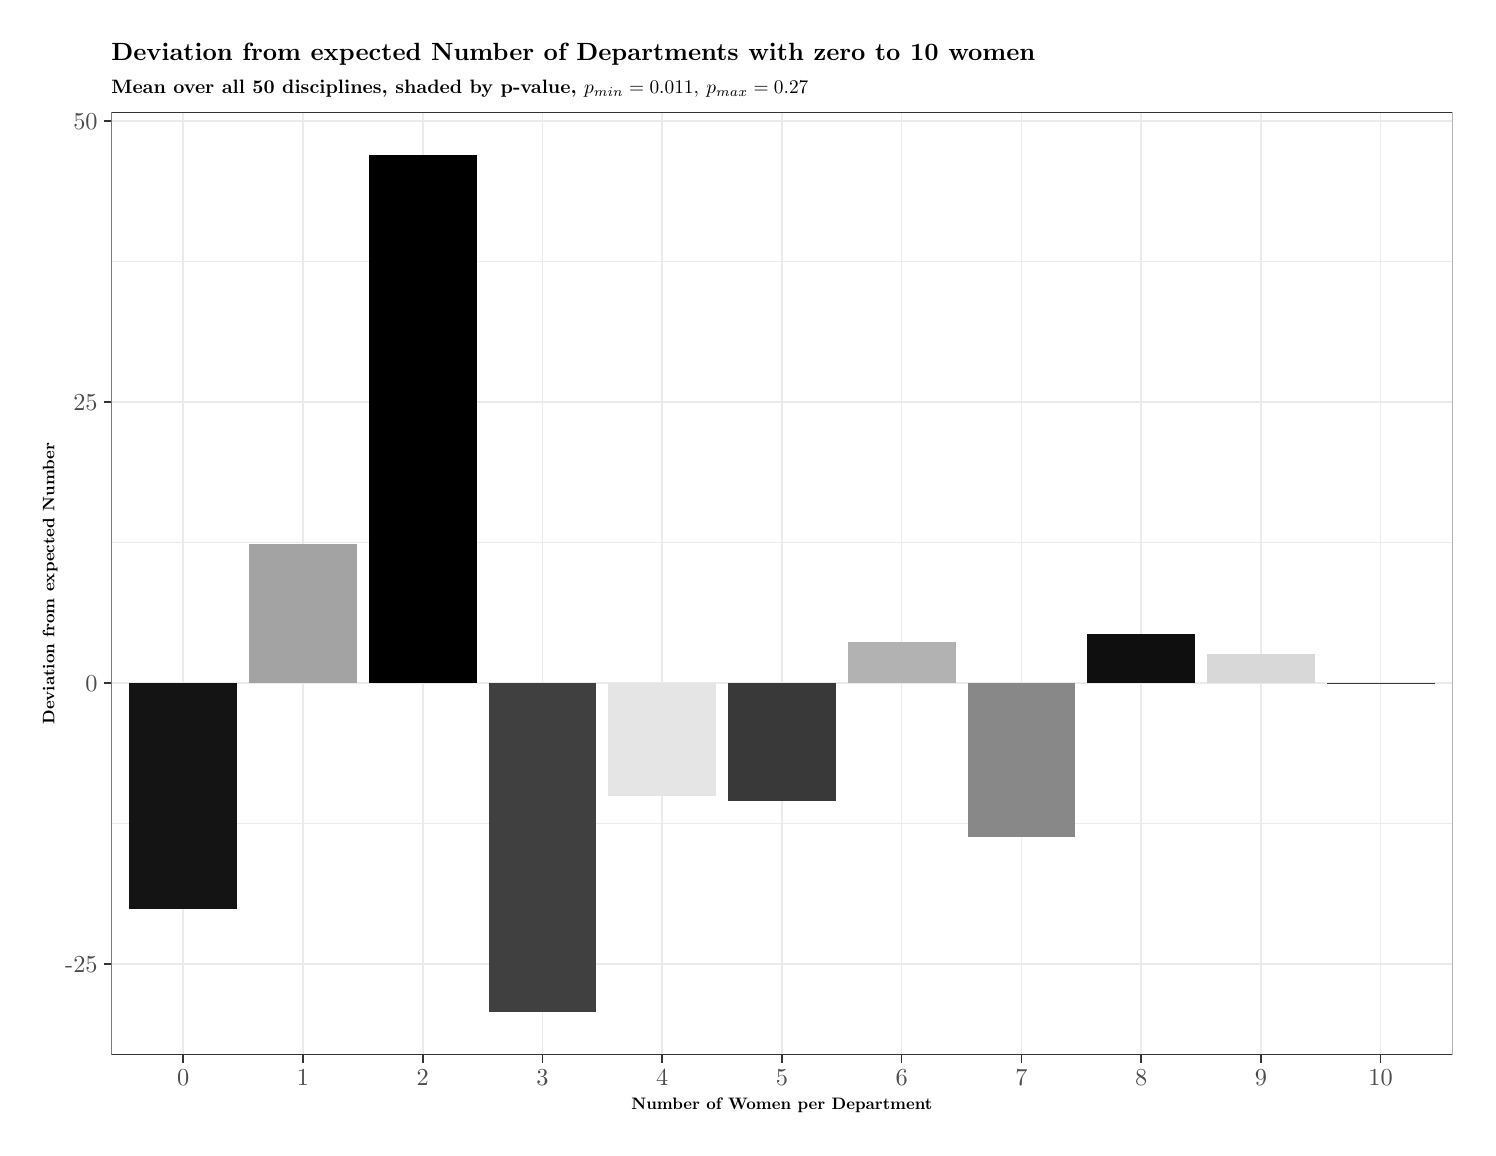
\begin{tikzpicture}[x=1pt,y=1pt]
\definecolor{fillColor}{RGB}{255,255,255}
\path[use as bounding box,fill=fillColor] (0,0) rectangle (520.34,397.48);
\begin{scope}
\path[clip] (  0.00,  0.00) rectangle (520.34,397.48);
\definecolor{drawColor}{RGB}{255,255,255}

\path[draw=drawColor,line width= 0.6pt,line join=round,line cap=round,fill=fillColor] (  0.00,  0.00) rectangle (520.34,397.48);
\end{scope}
\begin{scope}
\path[clip] ( 30.24, 26.28) rectangle (514.84,366.83);
\definecolor{fillColor}{RGB}{255,255,255}

\path[fill=fillColor] ( 30.24, 26.28) rectangle (514.84,366.83);
\definecolor{drawColor}{gray}{0.92}

\path[draw=drawColor,line width= 0.3pt,line join=round] ( 30.24,109.90) --
	(514.84,109.90);

\path[draw=drawColor,line width= 0.3pt,line join=round] ( 30.24,211.45) --
	(514.84,211.45);

\path[draw=drawColor,line width= 0.3pt,line join=round] ( 30.24,313.01) --
	(514.84,313.01);

\path[draw=drawColor,line width= 0.6pt,line join=round] ( 30.24, 59.12) --
	(514.84, 59.12);

\path[draw=drawColor,line width= 0.6pt,line join=round] ( 30.24,160.68) --
	(514.84,160.68);

\path[draw=drawColor,line width= 0.6pt,line join=round] ( 30.24,262.23) --
	(514.84,262.23);

\path[draw=drawColor,line width= 0.6pt,line join=round] ( 30.24,363.79) --
	(514.84,363.79);

\path[draw=drawColor,line width= 0.6pt,line join=round] ( 56.20, 26.28) --
	( 56.20,366.83);

\path[draw=drawColor,line width= 0.6pt,line join=round] ( 99.47, 26.28) --
	( 99.47,366.83);

\path[draw=drawColor,line width= 0.6pt,line join=round] (142.74, 26.28) --
	(142.74,366.83);

\path[draw=drawColor,line width= 0.6pt,line join=round] (186.00, 26.28) --
	(186.00,366.83);

\path[draw=drawColor,line width= 0.6pt,line join=round] (229.27, 26.28) --
	(229.27,366.83);

\path[draw=drawColor,line width= 0.6pt,line join=round] (272.54, 26.28) --
	(272.54,366.83);

\path[draw=drawColor,line width= 0.6pt,line join=round] (315.81, 26.28) --
	(315.81,366.83);

\path[draw=drawColor,line width= 0.6pt,line join=round] (359.08, 26.28) --
	(359.08,366.83);

\path[draw=drawColor,line width= 0.6pt,line join=round] (402.35, 26.28) --
	(402.35,366.83);

\path[draw=drawColor,line width= 0.6pt,line join=round] (445.61, 26.28) --
	(445.61,366.83);

\path[draw=drawColor,line width= 0.6pt,line join=round] (488.88, 26.28) --
	(488.88,366.83);
\definecolor{fillColor}{gray}{0.08}

\path[fill=fillColor] ( 36.73, 79.09) rectangle ( 75.67,160.68);
\definecolor{fillColor}{gray}{0.64}

\path[fill=fillColor] ( 80.00,160.68) rectangle (118.94,210.83);
\definecolor{fillColor}{RGB}{0,0,0}

\path[fill=fillColor] (123.26,160.68) rectangle (162.21,351.35);
\definecolor{fillColor}{gray}{0.25}

\path[fill=fillColor] (166.53, 41.76) rectangle (205.47,160.68);
\definecolor{fillColor}{gray}{0.90}

\path[fill=fillColor] (209.80,119.80) rectangle (248.74,160.68);
\definecolor{fillColor}{RGB}{57,57,57}

\path[fill=fillColor] (253.07,118.18) rectangle (292.01,160.68);
\definecolor{fillColor}{gray}{0.70}

\path[fill=fillColor] (296.34,160.68) rectangle (335.28,175.57);
\definecolor{fillColor}{RGB}{136,136,136}

\path[fill=fillColor] (339.61,105.04) rectangle (378.55,160.68);
\definecolor{fillColor}{gray}{0.06}

\path[fill=fillColor] (382.88,160.68) rectangle (421.82,178.29);
\definecolor{fillColor}{RGB}{216,216,216}

\path[fill=fillColor] (426.14,160.68) rectangle (465.09,171.19);
\definecolor{fillColor}{RGB}{58,58,58}

\path[fill=fillColor] (469.41,160.43) rectangle (508.35,160.68);
\definecolor{drawColor}{gray}{0.20}

\path[draw=drawColor,line width= 0.6pt,line join=round,line cap=round] ( 30.24, 26.28) rectangle (514.84,366.83);
\end{scope}
\begin{scope}
\path[clip] (  0.00,  0.00) rectangle (520.34,397.48);
\definecolor{drawColor}{gray}{0.30}

\node[text=drawColor,anchor=base east,inner sep=0pt, outer sep=0pt, scale=  0.88] at ( 25.29, 56.09) {-25};

\node[text=drawColor,anchor=base east,inner sep=0pt, outer sep=0pt, scale=  0.88] at ( 25.29,157.65) {0};

\node[text=drawColor,anchor=base east,inner sep=0pt, outer sep=0pt, scale=  0.88] at ( 25.29,259.20) {25};

\node[text=drawColor,anchor=base east,inner sep=0pt, outer sep=0pt, scale=  0.88] at ( 25.29,360.76) {50};
\end{scope}
\begin{scope}
\path[clip] (  0.00,  0.00) rectangle (520.34,397.48);
\definecolor{drawColor}{gray}{0.20}

\path[draw=drawColor,line width= 0.6pt,line join=round] ( 27.49, 59.12) --
	( 30.24, 59.12);

\path[draw=drawColor,line width= 0.6pt,line join=round] ( 27.49,160.68) --
	( 30.24,160.68);

\path[draw=drawColor,line width= 0.6pt,line join=round] ( 27.49,262.23) --
	( 30.24,262.23);

\path[draw=drawColor,line width= 0.6pt,line join=round] ( 27.49,363.79) --
	( 30.24,363.79);
\end{scope}
\begin{scope}
\path[clip] (  0.00,  0.00) rectangle (520.34,397.48);
\definecolor{drawColor}{gray}{0.20}

\path[draw=drawColor,line width= 0.6pt,line join=round] ( 56.20, 23.53) --
	( 56.20, 26.28);

\path[draw=drawColor,line width= 0.6pt,line join=round] ( 99.47, 23.53) --
	( 99.47, 26.28);

\path[draw=drawColor,line width= 0.6pt,line join=round] (142.74, 23.53) --
	(142.74, 26.28);

\path[draw=drawColor,line width= 0.6pt,line join=round] (186.00, 23.53) --
	(186.00, 26.28);

\path[draw=drawColor,line width= 0.6pt,line join=round] (229.27, 23.53) --
	(229.27, 26.28);

\path[draw=drawColor,line width= 0.6pt,line join=round] (272.54, 23.53) --
	(272.54, 26.28);

\path[draw=drawColor,line width= 0.6pt,line join=round] (315.81, 23.53) --
	(315.81, 26.28);

\path[draw=drawColor,line width= 0.6pt,line join=round] (359.08, 23.53) --
	(359.08, 26.28);

\path[draw=drawColor,line width= 0.6pt,line join=round] (402.35, 23.53) --
	(402.35, 26.28);

\path[draw=drawColor,line width= 0.6pt,line join=round] (445.61, 23.53) --
	(445.61, 26.28);

\path[draw=drawColor,line width= 0.6pt,line join=round] (488.88, 23.53) --
	(488.88, 26.28);
\end{scope}
\begin{scope}
\path[clip] (  0.00,  0.00) rectangle (520.34,397.48);
\definecolor{drawColor}{gray}{0.30}

\node[text=drawColor,anchor=base,inner sep=0pt, outer sep=0pt, scale=  0.88] at ( 56.20, 15.27) {0};

\node[text=drawColor,anchor=base,inner sep=0pt, outer sep=0pt, scale=  0.88] at ( 99.47, 15.27) {1};

\node[text=drawColor,anchor=base,inner sep=0pt, outer sep=0pt, scale=  0.88] at (142.74, 15.27) {2};

\node[text=drawColor,anchor=base,inner sep=0pt, outer sep=0pt, scale=  0.88] at (186.00, 15.27) {3};

\node[text=drawColor,anchor=base,inner sep=0pt, outer sep=0pt, scale=  0.88] at (229.27, 15.27) {4};

\node[text=drawColor,anchor=base,inner sep=0pt, outer sep=0pt, scale=  0.88] at (272.54, 15.27) {5};

\node[text=drawColor,anchor=base,inner sep=0pt, outer sep=0pt, scale=  0.88] at (315.81, 15.27) {6};

\node[text=drawColor,anchor=base,inner sep=0pt, outer sep=0pt, scale=  0.88] at (359.08, 15.27) {7};

\node[text=drawColor,anchor=base,inner sep=0pt, outer sep=0pt, scale=  0.88] at (402.35, 15.27) {8};

\node[text=drawColor,anchor=base,inner sep=0pt, outer sep=0pt, scale=  0.88] at (445.61, 15.27) {9};

\node[text=drawColor,anchor=base,inner sep=0pt, outer sep=0pt, scale=  0.88] at (488.88, 15.27) {10};
\end{scope}
\begin{scope}
\path[clip] (  0.00,  0.00) rectangle (520.34,397.48);
\definecolor{drawColor}{RGB}{0,0,0}

\node[text=drawColor,anchor=base,inner sep=0pt, outer sep=0pt, scale=  0.60] at (272.54,  6.67) {\bfseries Number of Women per Department};
\end{scope}
\begin{scope}
\path[clip] (  0.00,  0.00) rectangle (520.34,397.48);
\definecolor{drawColor}{RGB}{0,0,0}

\node[text=drawColor,rotate= 90.00,anchor=base,inner sep=0pt, outer sep=0pt, scale=  0.60] at (  9.64,196.56) {\bfseries Deviation from expected Number};
\end{scope}
\begin{scope}
\path[clip] (  0.00,  0.00) rectangle (520.34,397.48);
\definecolor{drawColor}{RGB}{0,0,0}

\node[text=drawColor,anchor=base west,inner sep=0pt, outer sep=0pt, scale=  0.70] at ( 30.24,373.69) {\bfseries Mean over all 50 disciplines, shaded by p-value, $p_{min}=0.011,$ $p_{max}=0.27$};
\end{scope}
\begin{scope}
\path[clip] (  0.00,  0.00) rectangle (520.34,397.48);
\definecolor{drawColor}{RGB}{0,0,0}

\node[text=drawColor,anchor=base west,inner sep=0pt, outer sep=0pt, scale=  0.90] at ( 30.24,385.77) {\bfseries Deviation from expected Number of Departments with zero to 10 women};
\end{scope}
\end{tikzpicture}
